\begin{figure}[htbp]
\centering
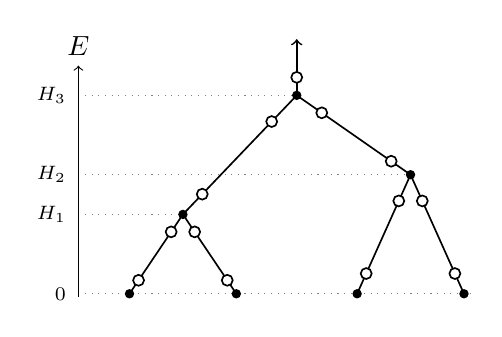
\begin{tikzpicture}[x=1.18cm,y=.84cm,
 endmark/.style={circle,draw,fill=white,inner sep=1.4pt}]
 \coordinate (a) at (0,0); \coordinate (b) at (1.15,0);
 \coordinate (c) at (2.45,0); \coordinate (d) at (3.60,0);
 \coordinate (u) at (.575,1.20); \coordinate (v) at (3.025,1.80);
 \coordinate (w) at (1.80,3.00);
 \draw[dotted,gray] (-.55,0) -- (3.70,0);
 \draw[dotted,gray] (-.55,1.20) -- (u);
 \draw[dotted,gray] (-.55,1.80) -- (v);
 \draw[dotted,gray] (-.55,3.00) -- (w);
 \foreach \start/\finish in {a/u,b/u,c/v,d/v,u/w,v/w}{
   \draw[semithick] (\start) -- node[endmark,pos=.17] {}
     node[endmark,pos=.78] {} (\finish);
 }
 \draw[semithick,->] (w) -- node[endmark,pos=.32] {} (1.80,3.85);
 \foreach \pt in {a,b,c,d,u,v,w}{\fill (\pt) circle[radius=1.7pt];}
 \draw[->] (-.55,-.05) -- (-.55,3.45) node[above] {\(E\)};
 \node[left,font=\scriptsize] at (-.58,0) {\(0\)};
 \node[left,font=\scriptsize] at (-.58,1.20) {\(H_1\)};
 \node[left,font=\scriptsize] at (-.58,1.80) {\(H_2\)};
 \node[left,font=\scriptsize] at (-.58,3.00) {\(H_3\)};
\end{tikzpicture}
\caption{Schematic of three saddle mergers for four wells at distinct heights \(H_1<H_2<H_3\). Edges represent maximal period annuli. Hollow circles mark the two finite ends of each bounded edge and the single finite end of the outer edge, thirteen in all. The lower bound for crossings near each marked end depends on its type and on the available modes in \eqref{eq:Bqalpha}.}
\label{fig:fold-geometry}
\end{figure}
